\documentclass[12pt,
               a4paper,
               article,
               oneside,
               english,oldfontcommands]{memoir}
\usepackage{student-kopi}
% Metadata
\date{\today}
\setmodule{MAT4110: Introduction to Numerical Analysis}
\setterm{Fall, 2023}

%-------------------------------%
% Other details
% TODO: Fill these
%-------------------------------%
\title{Mandatory assingment: 1}
\setmembername{Jonas Semprini Næss}  % Fill group member names

%-------------------------------%
% Add / Delete commands and packages
% TODO: Add / Delete here as you need
%-------------------------------%
\makeatletter
\newcommand*{\rom}[1]{\expandafter\@slowromancap\romannumeral #1@}
\makeatother
%\usepackage[utf8]{inputenc}
\usepackage{setspace}
\usepackage[T1]{fontenc}
\usepackage{titling}% the wheel somebody else kindly made for us earlier
\usepackage{fancyhdr}
\usepackage{fancybox}
\usepackage{epigraph} 
\usepackage{tikz}
\usepackage{bm}
\usepackage{pgfplots}
\pgfplotsset{compat=1.12}
\usepackage{lmodern}
\usepackage{enumitem}
\usepackage{framed}
\usepackage{calc}
\usepackage[labelfont=bf]{caption}
\usepackage{subcaption}
\usepackage{fancyvrb}
\usepackage[scaled]{beramono}
\usepackage[final]{microtype}
\usepackage{amssymb}
\usepackage{mathtools}
\usepackage{amsthm}
\usepackage{thmtools}
\usepackage{babel}
\usepackage{csquotes}
\usepackage{listings}
\usetikzlibrary{calc,intersections,through,backgrounds}
\usepackage{tkz-euclide} 
\lstset{basicstyle = \ttfamily}
\usepackage{float}
\usepackage{textcomp}
\usepackage{siunitx}
\usepackage{xcolor}
\usepackage{graphicx}
\usepackage[colorlinks, allcolors = uiolink]{hyperref}
\usepackage[noabbrev]{cleveref}
\pretolerance = 2000
\tolerance    = 6000
\hbadness     = 6000
\newcounter{probnum}[section]
\newcounter{subprobnum}[probnum] 
\usepackage{dirtytalk}
\usepackage{listings}
\usepackage{xcolor}
\usepackage{caption}
\usepackage[section]{placeins}
\usepackage{varwidth}
\usepackage{optidef}
\definecolor{uiolink}{HTML}{0B5A9D}
\usepackage[linesnumbered,ruled,vlined]{algorithm2e}
\usepackage{commath}
\newtheorem{theorem}{Theorem}[section]
\newtheorem{corollary}{Corollary}[theorem]
\newcommand{\Q}{ \qquad \hfill \blacksquare}
\newcommand\myeq{\stackrel{\mathclap{\normalfont{uif}}}{\sim}}
\let\oldref\ref
\renewcommand{\ref}[1]{(\oldref{#1})}
\newtheorem{lemma}[theorem]{Lemma}
\setlength \epigraphwidth {\linewidth}
\setlength \epigraphrule {0pt}
\AtBeginDocument{\renewcommand {\epigraphflush}{center}}
\renewcommand {\sourceflush} {center}
\parindent 0ex
\renewcommand{\thesection}{\roman{section}} 
\renewcommand{\thesubsection}{\thesection.\roman{subsection}}
\newcommand{\KL}{\mathrm{KL}}
\newcommand{\R}{\mathbb{R}}
\newcommand{\E}{\mathbb{E}}
\newcommand{\T}{\top}
\newcommand{\bl}{\left\{}
\newcommand{\br}{\right\}}
\newcommand{\spaze}{\vspace{4mm}\\}
\newcommand{\N}{\mathbb{N}}
\newcommand{\Rel}{\mathbb{R}}
\newcommand{\expdist}[2]{%
        \normalfont{\textsc{Exp}}(#1, #2)%
    }
\newcommand{\expparam}{\bm \lambda}
\newcommand{\Expparam}{\bm \Lambda}
\newcommand{\natparam}{\bm \eta}
\newcommand{\Natparam}{\bm H}
\newcommand{\sufstat}{\bm u}

\newlength{\MaxSizeOfLineNumbers}%
\settowidth{\MaxSizeOfLineNumbers}{99}% Adjust to maximum number of lines
\addtolength{\MaxSizeOfLineNumbers}{2.5ex}%

\definecolor{commentgreen}{RGB}{2,112,10}
\definecolor{weborange}{RGB}{255,165,0}
\definecolor{frenchplum}{RGB}{129,20,83}

\lstdefinestyle{mystyle}{  
	numbers=left, 
	numberstyle=\small, 
	numbersep=8pt, 
	frame=shadowbox,
	framexleftmargin=15pt,
	rulesepcolor=\color{gray},,
	linewidth=17.7cm,
  	language=python,
    tabsize=4,
    showstringspaces=false,
    numbers=left,
    %upquote=true,
    commentstyle=\color{commentgreen},
      keywordstyle=\color{blue},
    stringstyle=\color{red},
    basicstyle=\small\ttfamily, % basic font setting
    emph={int,char,double,float,unsigned,void,bool},
    emphstyle={\color{blue}},
    escapechar=\&,
    % keyword highlighting
    classoffset=1, % starting new class
    otherkeywords={>,<,.,;,-,!,=,~},
    morekeywords={>,<,.,;,-,!,=,~},
    keywordstyle=\color{purple},
    classoffset=0,
    morecomment=[s][\color{red}]{/*-}{*/}
}

\lstset{style=mystyle}

% Main document
\begin{document}
\header{}
\section*{\centering Problem 1.}
a.) \emph{Find a Householder transformation $H$ such that $B = HAH^T$ is a tridiagonal matrix. This involves some bookkeeping, so it may help to use the aid of a computer for calculating the linear algebra in steps that you describe.} \spaze
\textbf{Solution:} \spaze 
We observe that $A \in \R^{3 \times 3}$, meaning there is only a single Householder iteration needed to obtain our Householder matrix $H$. This is due to the Householder method only requiring $n-2$ reflection transformations to obtain the designated tridiagonal matrix, where $n$ naturally is the dimension of $A$. \vspace{2mm}\\ 
Now let $\bm{v} = \bm{x} + \text{sign}({x_{21}} )\bm{e}_1$ where $\bm{x} = [0, 1 / \sqrt{2},-1 / \sqrt{2}]^T$, which yields 
\begin{align*}
\bm{v} = \left[0, \frac{1 + \sqrt{2}}{\sqrt{2}},  -\frac{1}{\sqrt{2}} \right]^T.
\end{align*}
Hence our Householder transformation looks accordingly 
\begin{align*}
H = I_{3} - 2 \frac{\bm{v} \bm{v}^T}{\bm{v}^T \bm{v}}.
\end{align*}
By calculation $\bm{v}^T \bm{v} = 0^2 + (\frac{1 + \sqrt{2}}{\sqrt{2}})^2 + -(\frac{1}{\sqrt{2}})^2 = 2 + \sqrt{2}$, meaning the expression now becomes 
\begin{align*}
H = I_{3} - \frac{2}{2 + \sqrt{2}} \bm{v} \bm{v}^T 
\end{align*}
whereby the outer product $\bm{v} \bm{v}^T$ then gives 
\begin{align*}
H =  I_{3} - \begin{pmatrix}
0 &0 & 0 \\[5pt]
0 & \frac{\sqrt{2} + 1}{\sqrt{2}} & -\frac{1}{\sqrt{2}} \\[5pt]
0 & -\frac{1}{\sqrt{2}} & \frac{\sqrt{2} -1}{\sqrt{2}} 
\end{pmatrix} = 
\begin{pmatrix}
1 & 0 & 0 \\[5pt]
0 & -\frac{1}{\sqrt{2}} & \frac{1}{\sqrt{2}} \\[5pt]
0 & \frac{1}{\sqrt{2}} & \frac{1}{\sqrt{2}}
\end{pmatrix}.
\end{align*}
Which is then our Householder matrix. \vspace{2mm}\\
To really verify that $H$ is the transformation we are looking for, we can further calculate the product $B = H A H^T$. 
\begin{align*}
B &= H A H^T = H A H  \qquad (\text{H is symmetric})\\[10pt]
&=\begin{pmatrix}
1 & 0 & 0 \\[5pt]
0 & -\frac{1}{\sqrt{2}} & \frac{1}{\sqrt{2}} \\[5pt]
0 & \frac{1}{\sqrt{2}} & \frac{1}{\sqrt{2}}
\end{pmatrix} 
\begin{pmatrix}
5 & \frac{1}{\sqrt{2}} &  -\frac{1}{\sqrt{2}} \\[5pt]
\frac{1}{\sqrt{2}} &\frac{5}{2} & \frac{7}{2} \\[5pt]
-\frac{1}{\sqrt{2}} & \frac{7}{2} & \frac{5}{2}
\end{pmatrix}
\begin{pmatrix}
1 & 0 & 0 \\[5pt]
0 & -\frac{1}{\sqrt{2}} & \frac{1}{\sqrt{2}} \\[5pt]
0 & \frac{1}{\sqrt{2}} & \frac{1}{\sqrt{2}}
\end{pmatrix}
\\[10pt]
&= 
\begin{pmatrix}
5 & -1 & 0 \\[5pt]
-1 & -1 & 0\\[5pt]
0 & 0 & 6
\end{pmatrix}
\end{align*}
where $B$ is a tridiagonal matrix. $\Q$ \spaze 
b.) \emph{Use Gershgorin’s second theorem in combination with a similarity transformation to estimate the spectrum of A. Show that all eigenvalues are distinct and describe the location of the eigenvalues as accurately as you can.} \spaze 
\textbf{Solution:} \spaze
By Gershgorin`s Circle Theorem we know that when approximating the eigenvalues of $A$, the respective eigenvalues has to lay within at least one of the discs 
\begin{align*}
D(a_{ii}, R_i) \subseteq \mathbb{C}.
\end{align*}
Where $a_{ii}$ are the diagonal elements of $A$ and $R_i = \sum_{j \neq i} |a_{ij}|$.\vspace{2mm}\\ By this result we can hence elaborate further on the eigenvalues of $A$ by observing the discs
\begin{align}
&D_{1}(5, \sqrt{2}) \\[5pt]
&D_{2} \left( \frac{5}{2}, \frac{7 + \sqrt{2}}{2} \right).
\end{align}
Since $D_1 \subseteq D_2 \Rightarrow D_1 \cap D_2 \neq \emptyset$ it becomes beneficial to dissect these discs even farther seeing we wish to have as many disjont discs possible \footnote{Direct consequence of Greshgorin`s second theorem stating that: \say{If the union of $k$ discs is disjoint from the union of the other $n-k$ discs then the former union contains exactly k and the latter $n-k$ eigenvalues of A, when the eigenvalues are counted with their algebraic multiplicities.}} To do so it is advantageous to perform a similarity transformation (looking into the same input space of $A$, but from the viewpoint of a different basis). Let
\begin{align*}
T = \begin{pmatrix}
1 & 0 & 0 \\[5pt]
0 & \alpha & 0 \\[5pt]
0 & 0 & 1
\end{pmatrix}
\end{align*}
for $\alpha > 0$ and notice that since $B$ from (a.) is simply a reflection transformation of $A$ the spectrum of $A$ is conserved. This means that 
\begin{align*}
\sigma(A) &=\sigma(HAH^T) \\[5pt]
&=\sigma(B) \\[5pt]
&= \sigma(T B T^{-1}).
\end{align*}
Thus, by taking the product $TBT^{-1}$ we have that 
\begin{align*}
TBT^{-1} &= \begin{pmatrix}
1 & 0 & 0 \\[5pt]
0 & \alpha & 0 \\[5pt]
0 & 0 & 1
\end{pmatrix}
\begin{pmatrix}
5 & -1 & 0 \\[5pt]
-1 & -1 & 0\\[5pt]
0 & 0 & 6
\end{pmatrix}
\begin{pmatrix}
1 & 0 & 0 \\[5pt]
0 & \frac{1}{\alpha} & 0 \\[5pt]
0 & 0 & 1
\end{pmatrix} \\[10pt]
&= \begin{pmatrix}
5 & -\frac{1}{\alpha}& 0 \\[5pt]
-\alpha & -1 & 0\\[5pt]
0 & 0 & 6
\end{pmatrix}
\end{align*}. 
Applying Greshgorin`s Circle Theorem again yields the following discs 
\begin{align}
\tilde{D}_{1}\left(5, \frac{1}{\alpha}\right) \\[5pt]
\tilde{D}_{2}\left( -1, \alpha \right).
\end{align}
Seeing that (from row 3) $|k - 6| \leq 0, \  k \in \mathbb{R}$ we can conclude with $\lambda_{1} = 6$ being one of the eigenvalues of $A$. Moreover, to hence determine the potential other eigenvalues we must demand that
\begin{align*}
\tilde{D}_{1} \cap \tilde{D}_{2} = \emptyset &\Rightarrow 5 - \frac{1}{\alpha} = -1 + \alpha\\[5pt]
&\Downarrow \\[5pt]
-\alpha^2 +&6 \alpha - 1 = 0.
\end{align*}
This systems has solutions $\alpha_{1} \approx 5.828427, \ \alpha_{2} \approx 0.1715728$, which yields $\lambda_{2} \in \tilde{D_{1}}(\alpha \approx 5.828427) = B((5, 0.1715716))$ and  $\lambda_{3} \in \tilde{D_{2}}(\alpha \approx 0.1715728) = B((-1,0.1715728))$, telling us that 
\begin{align*}
\lambda_2 &\in [5 - 0.1715716, 5 + 0.1715716] \\[5pt]
\lambda_3 &\in [-1- 0.1715728, -1 + 0.1715728].
\end{align*}
\begin{figure}[H]
\centering 
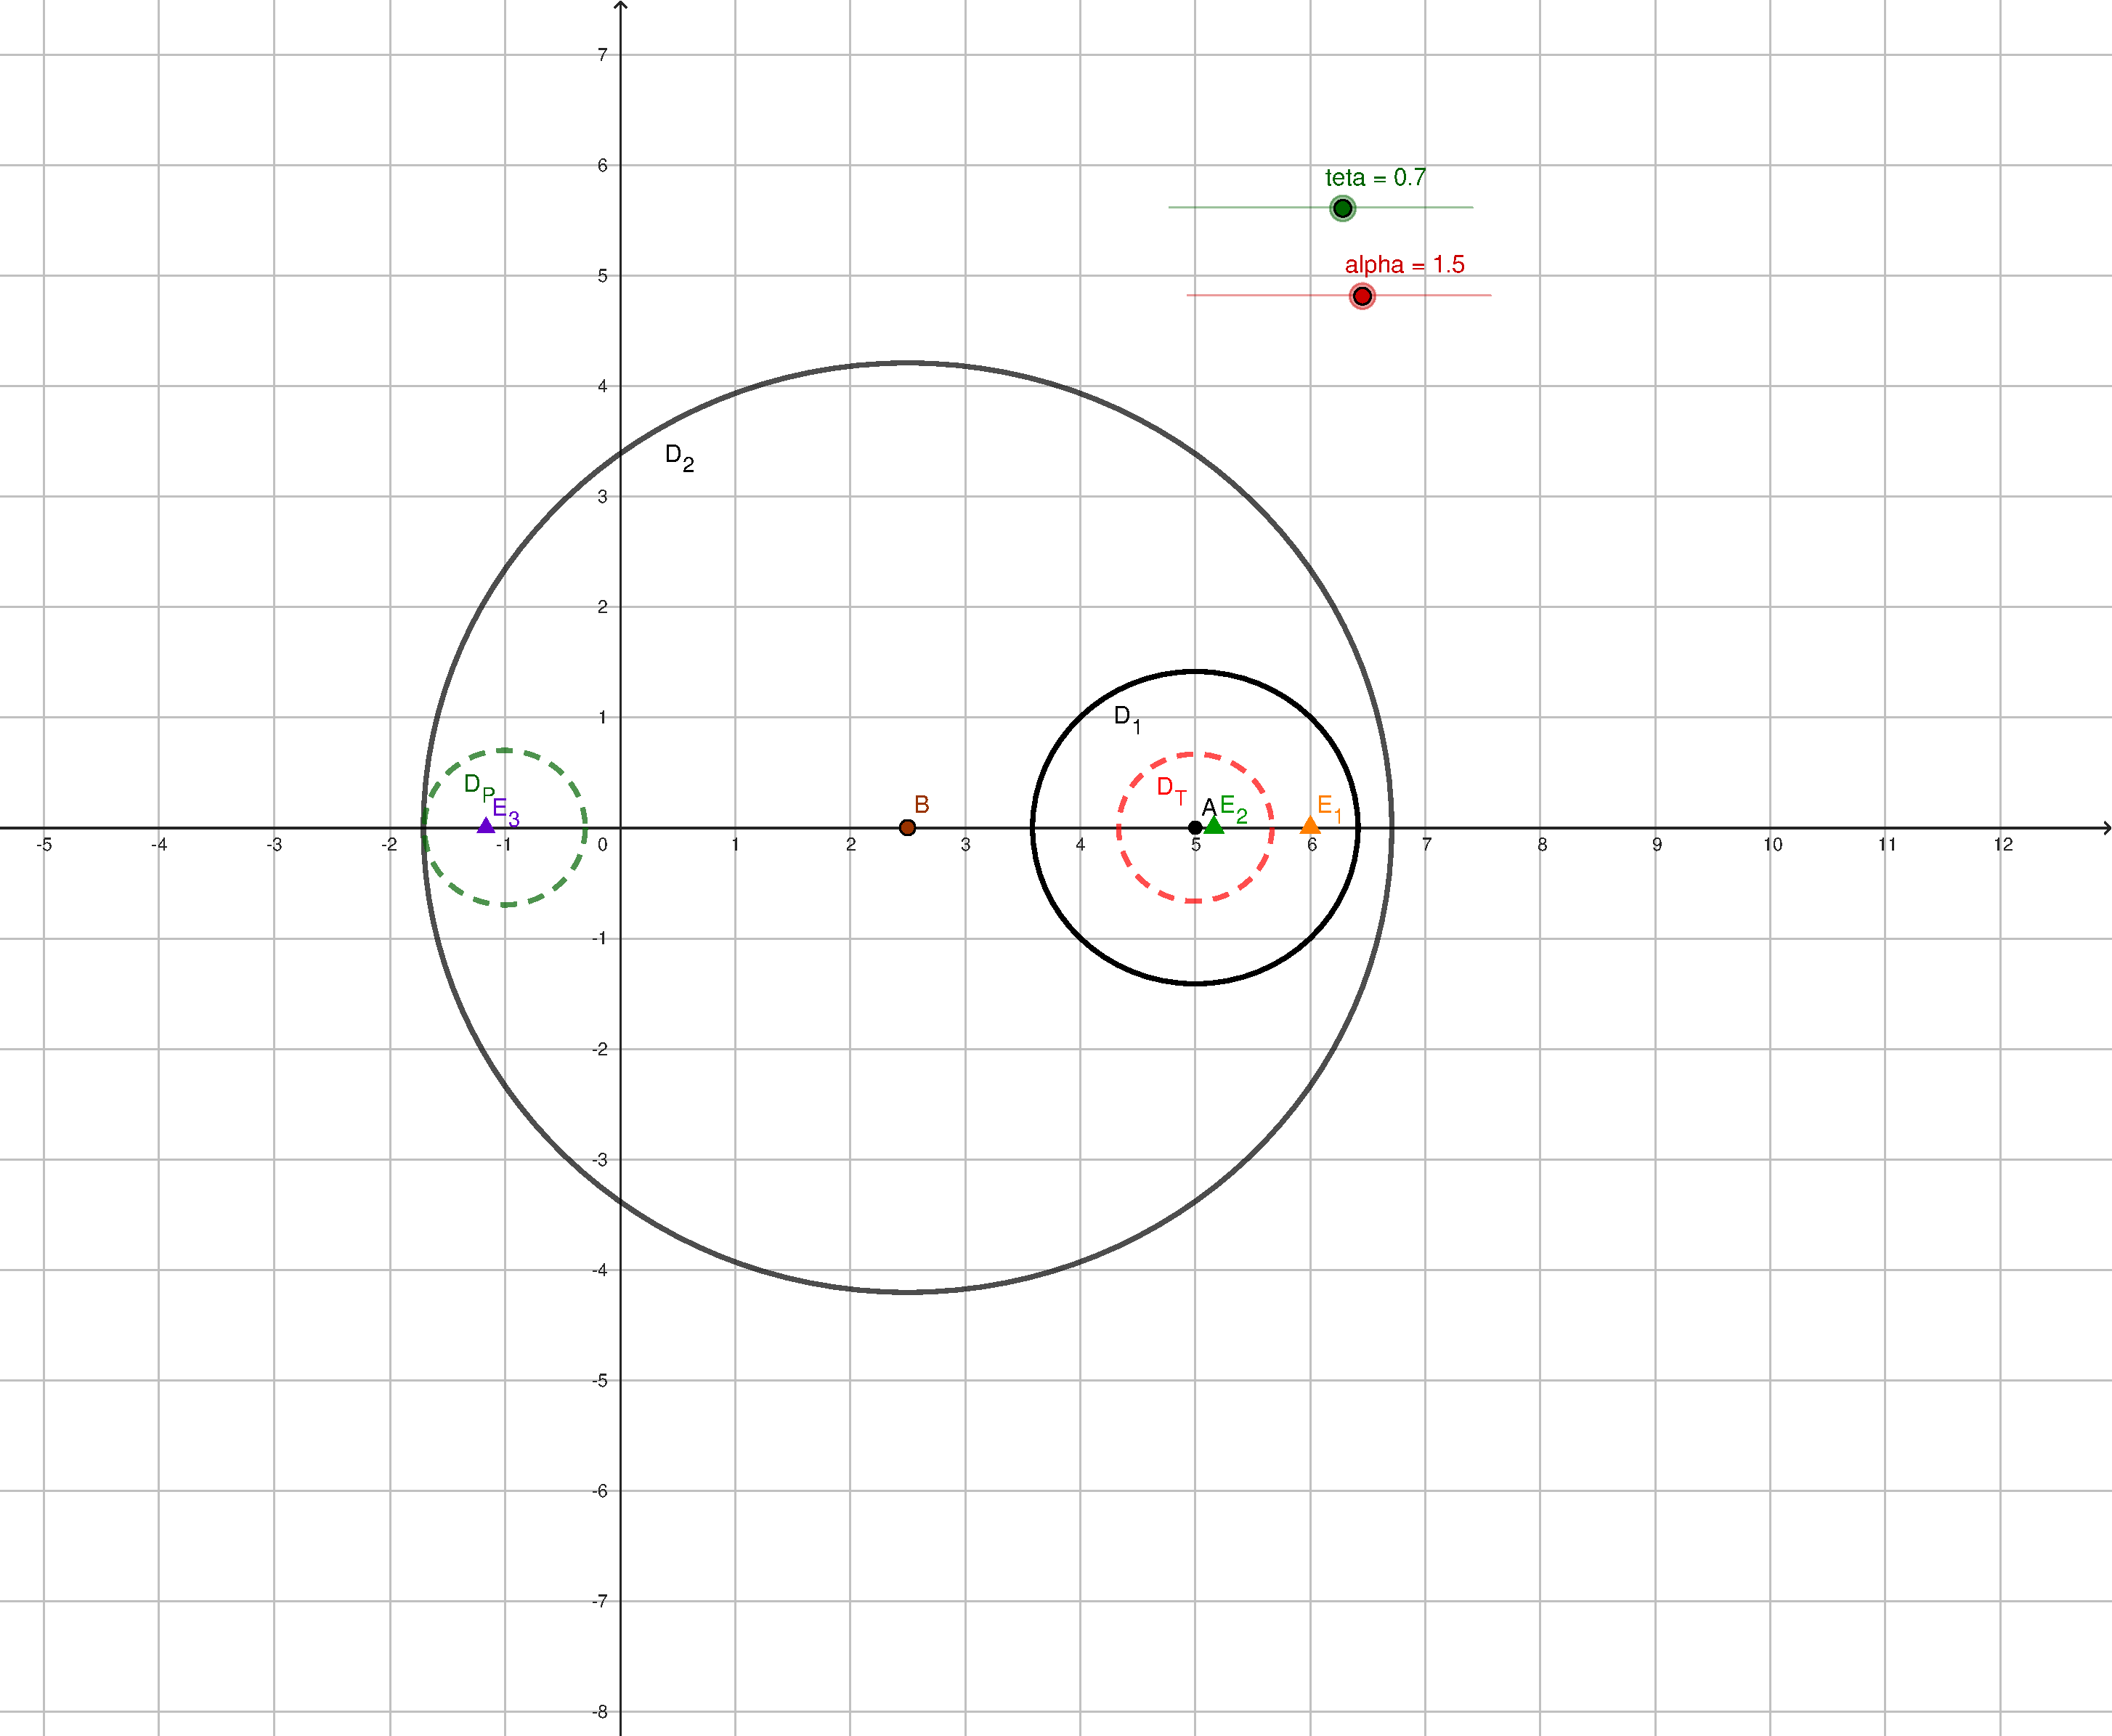
\includegraphics[width=1\textwidth]{exercise_1_b.pdf}
\caption{Visual of the Greshgorin circles. $D_1, D_2$ (Black) are the discs corresponding to $A$, $E_1, E_2, E_3$ are the actual eigenvalues of $A$, $D_T, D_P$ the discs corresponding to $TBT^{-1}$ and $\alpha_{1} = 1.5, \ \alpha_2 = 0.7$}
\end{figure}
c.) \emph{Computer exercise: Approximate the largest eigenvalue of A using power iteration and approximate the other two eigenvalues with inverse iteration (a shift is needed for the middle eigenvalue). Draw a random vector $x^{(0)}$ as start vector (for instance, with the components being independent, standard normal distributed). Include your implementation code and the output of 10 iterations for each approximation.} \spaze 
\textbf{Solution:} \spaze 
By running the implemented power iteration over $10$ iterations through script \ref{lst: power} the following ouput is given 
\begin{table}[H] 
  \begin{center} 
    \label{tab: power it}
    \begin{tabular}{c c c } 
      \textbf{Approx Eigenvalue}& \textbf{Actual Eigenvalue} & \textbf{Error}\\
      \hline 
      	6.0800585  &     6.0 & 0.0800585\\
      	 5.6356824      &          6.0  & 0.3643176\\
         5.7005412        &        6.0  &0.2994588\\
          5.7557640         &     6.0  &0.2442360\\
          5.8043507        &        6.0&  0.1956493\\
          5.8457834         &       6.0  & 0.1542166\\
          5.8800852          &      6.0 & 0.1199148\\
         5.9077903           &     6.0  &0.0922097\\
         5.9297235              &  6.0 & 0.0702765\\
       5.9468134              &  6.0 & 0.0531866\\
      \hline
    \end{tabular}
     \caption{Output through 10 iterations of the power iteration.}
  \end{center}
\end{table}
For inverse iteration the following is given 
\begin{table}[H] 
  \begin{center} 
    \label{tab: inv it}
    \begin{tabular}{c c c } 
      \textbf{Approx Eigenvalue}& \textbf{Actual Eigenvalue} & \textbf{Error}\\
      \hline 
        1.0000000   &      -1.1622777  &2.1622777\\
       4.6485161         &-1.1622777  &5.8107938\\
       -6.1464352         &-1.1622777  &4.9841576\\
       -0.7073727        & -1.1622777  &0.4549050\\
          -1.2235930        & -1.1622777  &0.0613154\\
          -1.1575017        & -1.1622777  &0.0047760\\
          -1.1616153         &-1.1622777  &0.0006624\\
          -1.1627635        & -1.1622777  &0.0004858\\
          -1.1621031         &-1.1622777  &0.0001746\\
          -1.1623296         &-1.1622777  &0.0000519\\
         -1.1622635         &-1.1622777  &0.0000141\\
      \hline
    \end{tabular}
     \caption{Output through 10 iterations of the inverse iteration.}
  \end{center}
\end{table}
and lastly for the shifted inverse iteration with $\mu = 5$. 
\begin{table}[H] 
  \begin{center} 
    \label{tab: inv shift}
    \begin{tabular}{c c c } 
      \textbf{Approx Eigenvalue}& \textbf{Actual Eigenvalue} & \textbf{Error}\\
      \hline 
           6.0000000     &     5.1622777 & 8.3772234e-01\\
          5.3504813        &  5.1622777 & 1.8820363e-01\\
           5.2036234       &   5.1622777  & 4.1345701e-02\\
           5.1691899         & 5.1622777  & 6.9122765e-03\\
           5.1634094        &  5.1622777 & 1.1317319e-03\\
           5.1624615         & 5.1622777  & 1.8380479e-04\\
           5.1623075         & 5.1622777 & 2.9834424e-05\\
           5.1622825        &  5.1622777 &  4.8415647e-06\\
           5.1622784          & 5.1622777 & 7.8568265e-07\\
           5.1622778         & 5.1622777 & 1.2749881e-07\\
          5.1622777          & 5.1622777 & 2.0690213e-08\\
      \hline
    \end{tabular}
     \caption{Output through 10 iterations of the inverse iteration with shift ($\mu = 5$).}
  \end{center}
\end{table}
\section*{\centering Problem 2.}
a.) \emph{Describe the function $R(\beta)$ for the nonlinear least
squares problem for determining this circle and compute its Jacobian $J_{R}(\beta) \in \R^{20 \times 3}$.} \spaze
\textbf{Solution:}\spaze
The function $R(\beta)$ is simply what is defined as the cost function. By taking the difference of the model(estimation) against the true measurement, you will acheive what is called a residual, or error margin, which describes how much the model deviates at that certain point. Therefore, can $R(\beta)$ look as follows 
\begin{align*}
R(\beta)=  \begin{bmatrix}
f(x_1, y_1; \beta) - b_1 \\[5pt] 
f(x_2, y_2; \beta) - b_2 \\[5pt]
\vdots \\[5pt]
f(x_n, y_n; \beta) - b_n
\end{bmatrix}
\end{align*}
which relative to this sample data gives 
\begin{align*}
R(\beta)=  \begin{bmatrix}
f(x_1, y_1; \beta) - b_1 \\[5pt] 
f(x_2 y_2; \beta) - b_2 \\[5pt]
\vdots \\[5pt]
f(x_{20}, y_{20}; \beta) - b_{20}
\end{bmatrix}.
\end{align*}
For the case of the Jacobian we remember that a general Jacobian is defined as 
\begin{align*}
J_{f} = \begin{bmatrix}
\frac{\partial f_1}{\partial x_1} &\ldots &\frac{\partial f_1}{\partial x_n} \\[5pt]
\vdots &\ddots & \vdots \\[5pt]
\frac{\partial f_m}{\partial x_1} &\ldots &\frac{\partial f_m}{\partial x_n} 
\end{bmatrix}
\end{align*}
where $f: \R^{n} \mapsto \R^{m}$ and $x \in \R^{n}$. Hence will the Jacobian for $f(x,y; \beta)$ look as follows 
\begin{align*}
J_{R}(\beta) &= \begin{bmatrix}
\frac{\partial f_1}{\partial \beta_1} &\ldots &\frac{\partial f_1}{\partial \beta_3} \\[5pt]
\vdots &\ddots & \vdots \\[5pt]
\frac{\partial f_{20}}{\partial x_1} &\ldots &\frac{\partial f_{20}}{\partial \beta_3} 
\end{bmatrix} \\[10pt]
&= \begin{bmatrix}
-2(x_1 - \beta_1) & -2(y_1 - \beta_2)& -2\beta_3\\[5pt]
\vdots & \vdots & \vdots\\[5pt]
 -2(x_{20} - \beta_1) &  -2(y_{20} - \beta_2) & -2\beta_3
\end{bmatrix} \\
\end{align*}
b.) \emph{Find a reasonable guess for $\beta^{0}$ and compute the circle $\beta^{*}$ that best describes the measurements in least squares sense using the Gauss-Newton method (3) on a computer. Include one plot of containing the circle $\beta^{*}$ you obtain and the measurement points.} \spaze 
\textbf{Solution:} \spaze
Code can be found be found in the Appendix at \ref{lst: ls circ}, and produces the following plot. \spaze
c.) \emph{Solve the linear least squares problem with unknowns $(x_c, y_c, w)$ on a computer and use the equation for $w$ to determine the circle`s radius, $r$. How does the solution of this linear least squares problem compare to what you obtained in part b)?}\spaze 
\textbf{Solution:}\spaze 
By rewriting the equation we can implement the linear least squares as 
\begin{align*}
2xx_c + 2yy_c + -x_{i}^2 - y_{i}^2 = 0
\end{align*}
which by the following code (\ref{lst: lls circ}) gives $r \approx 3.690027147759961$, which aligns well with the results of $\beta_3$ from (b.).
\section*{\centering Problem 3.}
a.) \emph{Describe $L_{k}(x)$ and $\hat{L}_{p}(y)$ and show that $p(x,y)$ in (7) with the functions $L_{k}(x)$ and $\hat{L}_{p}(y)$ that you define indeed is a solution of (6).} \spaze
 \textbf{Solution:} \spaze 
 We know by the ridgid definition of the Lagrange Polynomial in one dimension that 
 \begin{align*}
 L_{k}(x) =   \prod_{\mathclap{\substack{i = 0\\
                              i \neq k \\}}}^{n} \frac{x - x_{i}}{x_k - x_i} = \frac{(x - x_0) (x - x_1 )\ldots( x- x_{i-1}) \ldots (x - x_n)}{(x_i - x_0)(x_i - x_1) \ldots (x_i - x_{i-1}) (x_i - x_{i+1}) \ldots (x_i - x_n)}
 \end{align*}
 which can also be generalised for $y$, in the same manner, implying that 
 \begin{align*}
\hat{L}_{p}(y) =  \prod_{\mathclap{\substack{j= 0\\
                              j \neq p \\}}}^{n} \frac{y - y_j}{y_p - y_j} =\frac{(y - y_0) (y - y_1 )\ldots( y- y_{j-1}) \ldots (y - y_n)}{(y_j - y_0)(y_j - y_1) \ldots (y_j - y_{j-1}) (y_j - y_{j+1}) \ldots (x_j - y_n)}
 \end{align*}
 Now observe for equation (6) that it becomes 
 \begin{align*}
 p(x_i,y_j) = \sum_{k=0}^{n}  \sum_{p=0}^{n} f(x_k, y_p) L_{k}(x_i) \hat{L}_{p}(y_j) &= \sum_{k=0}^{n}  \sum_{p=0}^{n} f(x_k, y_p) \delta_{ik} \delta_{jp}, \quad i \neq k \land j\neq p. \\[5pt]
 &= f(x_i, y_j)
 \end{align*}
 which means that it interpolates the data, since each basis polynomial has degree $n$ and hence must the sum (or linear combinations) be of degree $\leq n$. Conclusively must $p(x,y)$ be a solution of $p(x_i. y_j) = f(x_i, y_j), \ \forall \ 0 \leq i,j \leq n$.  $\Q$ \spaze
b.) \emph{Leaning on the fact that any univariate polynomial $p$ of degree $ \leq n$ that has $n + 1$ or more zeros is equal to the 0 function, meaning $ p \equiv 0$, show that the solution to the 2 dimensional interpolation problem (6) is unique.}\spaze 
\textbf{Solution:} \spaze
Suppose that $p$ is not unique and there exists another solution to the interplolation problem $q \in \mathcal{P}_{n,n}$. Now define $r = p - q$, implying that $r \in \mathcal{P}_{n,n}$, meaning we can write it as 
\begin{align*}
\sum_{i=0}^{n}\sum_{j=0}^{n} c_{i,j}x^{i}y^{j}, \ c_{i,j} \in \mathbb{R}.
\end{align*}
Without loss of generality, we can fix any $ 0 \leq p \leq n$ such that the function $r(x, y_p)$ is now a univariate polyomial in $x$ of degree $\leq n$ and can be written as
\begin{align*}
\sum_{i=0}^{n} a_{i}(y_p)x^{i}
\end{align*} 
where $  a_{i}(y_p) = \sum_{j=0}^{n} c_{i,j} y_{p}^{j}$.  This polynomial has $n+1$ distinct root, namely $x_i, \ i=0, 1, \ldots, n$. But a polynomial that has $n+1$ distinct roots and is of degree $\leq n$ can only happen to exist as long its $\equiv 0$ , which tells us that the only solution to $r(x, y_p) = 0 $ is if all $a_{i}(y_p) = 0 \iff c_{i,j} =0, \ \forall i,j$ meaning $r(x,y) \equiv 0$, which contradicts our assumption and $p \in \mathcal{P}$ must therefore be unique. $\Q$\spaze
c.) \emph{Determine $p_{i,j}(x,y)$ and verify that the 2D square-mesh trapezoidal rule is given by}
\begin{align*}
T(n) = \frac{h^2}{4}\sum_{i=1}^{n}\sum_{j=1}^{n} \left( f(x_{i-1}, y_{j-1}) + f(x_i, y_{j-1}) +  f(x_{i-1}, y_{j-1}) +  f(x_i, y_{j}) \right)
\end{align*}
\textbf{Solution:} \spaze
d.) \emph{ For $n^s = 2^{1+s}, \ s = 1,2, \ldots, 7$ compute $T(n^s)$ to estimate the integral}
\begin{align*}
I = \int_{0}^{1} \int_{0}^{1} \text{exp}(-(x - \sin(y^2))^3) \ dx \ dy
\end{align*}
\emph{Estimate numerically the order of convergence r in}
\begin{align*}
E(n) = cn^{-r} + \mathcal{O}(n^{-(r+1)})
\end{align*}
\textbf{Solution:} \spaze
\section*{\centering \underline{Appendix}}
\subsubsection*{\centering Source code}
\begin{lstlisting}[caption= Power Iteration, label={lst: power}]
import numpy as np
import pandas as pd
import random

matrix = np.array(
    [
        [5, 1 / np.sqrt(2), -1 / np.sqrt(2)],
        [1 / np.sqrt(2), 5 / 2, 7 / 2],
        [-1 / np.sqrt(2), 7 / 2, 5 / 2],
    ]
)

result = pd.DataFrame(columns=["Approx Eigenvalue", "Actual Eigenvalue", "Error"])

num_iterations = 10
actual_eigenvalues, _ = np.linalg.eig(matrix)
print(actual_eigenvalues)
actual_largest_eigenvalue = max(actual_eigenvalues)

n = matrix.shape[0]
b = np.random.rand(n)

for i in range(num_iterations):
    # Power iteration
    b = np.dot(matrix, b)
    # Normalize the vector
    eigenvalue = np.linalg.norm(b)
    error = abs(eigenvalue - actual_largest_eigenvalue)
    b /= eigenvalue
    result.loc[i] = [eigenvalue, actual_largest_eigenvalue, error]


with pd.option_context(
    "display.max_rows",
    None,
    "display.max_columns",
    None
\end{lstlisting}

\begin{lstlisting}[caption= Inverse Iteration, label={lst: inverse}]
import numpy as np
import pandas as pd
import random

matrix = np.array(
    [
        [5, 1 / np.sqrt(2), -1 / np.sqrt(2)],
        [1 / np.sqrt(2), 5 / 2, 7 / 2],
        [-1 / np.sqrt(2), 7 / 2, 5 / 2],
    ]
)

result = pd.DataFrame(columns=["Approx Eigenvalue", "Actual Eigenvalue", "Error"])

num_iterations = 10
actual_eigenvalues, _ = np.linalg.eig(matrix)


def inverse_power_method(matrix, iter, tol=1e-15):
    A = matrix
    b = np.zeros((len(A), iter + 1))
    b[:, 0] = np.random.normal(0, 0.1, A.shape[0])
    rn = np.ones((iter + 1,))
    for k in range(num_iterations):
        b[:, k] = b[:, k] / np.linalg.norm(b[:, k])
        b[:, k + 1] = np.linalg.solve(A, b[:, k])
        rn[k + 1] = np.sum(b[:, k + 1]) / np.sum(b[:, k])
        if abs(rn[k + 1] - rn[k]) < tol:
            break
    if k < iter:
        rn[k + 2 :] = rn[k + 1]
    inv_pow = 1.0 / rn
    for i in range(0, len(inv_pow)):
        eigenvalue = inv_pow[i]
        error = abs(eigenvalue - actual_eigenvalues[1])
        result.loc[i] = [eigenvalue, actual_eigenvalues[1], error]



inverse_power_method(matrix, iter=num_iterations)

with pd.option_context(
    "display.max_rows",
    None,
    "display.max_columns",
    None,
    "display.precision",
    7,
):
    print(result)
\end{lstlisting}

\begin{lstlisting}[caption= Inverse Iteration with shift, label={lst: inv shift}]
import numpy as np
import pandas as pd
import random

matrix = np.array(
    [
        [5, 1 / np.sqrt(2), -1 / np.sqrt(2)],
        [1 / np.sqrt(2), 5 / 2, 7 / 2],
        [-1 / np.sqrt(2), 7 / 2, 5 / 2],
    ]
)

result = pd.DataFrame(columns=["Approx Eigenvalue", "Actual Eigenvalue", "Error"])

num_iterations = 10
actual_eigenvalues, _ = np.linalg.eig(matrix)

def inverse_power_method(matrix, mu, iter, tol=1e-15):
    Ashift = matrix - mu * np.identity(matrix.shape[0])
    b = np.zeros((len(Ashift), iter + 1))
    b[:, 0] = np.random.normal(0.5, 0.3, Ashift.shape[0])
    rn = np.ones((iter + 1,))
    for k in range(num_iterations):
        b[:, k] = b[:, k] / np.linalg.norm(b[:, k])
        b[:, k + 1] = np.linalg.solve(Ashift, b[:, k])
        rn[k + 1] = np.sum(b[:, k + 1]) / np.sum(b[:, k])
        if abs(rn[k + 1] - rn[k]) < tol:
            break
    if k < iter:
        rn[k + 2 :] = rn[k + 1]
    inv_pow = 1.0 / rn + mu
    for i in range(0, len(inv_pow)):
        eigenvalue = inv_pow[i]
        error = abs(eigenvalue - actual_eigenvalues[0])
        result.loc[i] = [eigenvalue, actual_eigenvalues[0], error]


mu = 5
inverse_power_method(matrix, mu, iter=num_iterations)

with pd.option_context(
    "display.max_rows",
    None,
    "display.max_columns",
    None,
    "display.precision",
    7,
):
    print(result)
\end{lstlisting}    
\begin{lstlisting}[caption= Least Squares fit Circle Fit, label={lst: ls circ}]
import scipy.io
import numpy as np
import matplotlib.pyplot as plt

measurementData = scipy.io.loadmat("circle-measurements.mat")
x = measurementData["x"].reshape(-1)
y = measurementData["y"].reshape(-1)

phi = np.linspace(0, 1, 100)

b_1 = (max(x) + min(x)) / 2
b_2 = (max(y) + min(y)) / 2
b_3 = (abs(max(x)) + abs(min(x)) + abs((max(y)) + abs(min(x)))) / 4
beta = [b_1, b_2, b_3]

n = 3
matrix = np.zeros((len(x), n))


def circle_model(beta, x, y):
    return (x - beta[0]) ** 2 + (y - beta[1]) ** 2 - beta[2] ** 2


def Jacobian(matrix, beta):
    jac = matrix
    for i in range(0, len(x)):
        jac[i][0] = -2 * (x[i] - beta[0])
        jac[i][1] = -2 * (y[i] - beta[1])
        jac[i][2] = -2 * (beta[2])
    return jac


def gauss_newton(beta, max_iter=100, tolerance=1e-6):
    params = beta
    for _ in range(max_iter):
        J = Jacobian(matrix, params)
        r = circle_model(params, x, y)
        J_T = np.transpose(J)
        S = np.linalg.pinv(np.matmul(J_T, J))
        delta_params = np.matmul(S, np.matmul(J_T, r))

        # print(delta_params.shape, r.shape)
        params = params - delta_params

        if np.linalg.norm(delta_params) < tolerance:
            break

    return params


beta_n = gauss_newton(beta)
print(beta_n)

s1 = beta_n[0] + beta_n[2] * np.cos(2 * np.pi * phi)
s2 = beta_n[1] + beta_n[2] * np.sin(2 * np.pi * phi)
plt.scatter(x, y, marker="o", color="green", label="Measure points")
plt.plot(s1, s2, color="red")
plt.xlim(min(x), max(x))
plt.ylim(min(y) - 1, max(y) + 2)
plt.legend()
 plt.show()
\end{lstlisting}
\begin{lstlisting}[caption= Linear Least Squares fit Circle Fitt, label={lst: lls circ}]
import scipy.io
import numpy as np
import matplotlib.pyplot as plt

measurementData = scipy.io.loadmat("circle-measurements.mat")
x = measurementData["x"].reshape(-1)
y = measurementData["y"].reshape(-1)

A = np.c_[2 * x, 2 * y, np.ones_like(x)]

r = np.linalg.solve(A.T @ A, A.T @ (-(x**2) - (y**2)))

r_fit = np.sqrt(r[0] ** 2 + r[1] ** 2 - r[2])

print(r_fit)
\end{lstlisting}
\end{document}